\documentclass[a4paper]{article}

%% Language and font encodings
\usepackage[english]{babel}
\usepackage[utf8x]{inputenc}
\usepackage[T1]{fontenc}

%% Sets page size and margins
\usepackage[a4paper,top=3cm,bottom=2cm,left=3cm,right=3cm,marginparwidth=1.75cm]{geometry}

%% Useful packages
\usepackage{amsmath}
\usepackage{graphicx}
\usepackage[colorinlistoftodos]{todonotes}
\usepackage[colorlinks=true, allcolors=blue]{hyperref}
\usepackage{lipsum}
\usepackage{todonotes}

\title{Thiazole paper name here}
\author{Authors here}

\begin{document}
\maketitle

\begin{abstract}
\lipsum[20]
\end{abstract}


\section{Introduction}

Thiazole ($\rm C_3H_3NS$) is an aromatic ring molecule, which can be percieved as a cyclopentadienyl ($\rm C_3H_3NS$) ring with one nitrogen and one sulphur substitutients at positions $1, 3$. The macroscopic chemical and physical properties of thiazole and its place among other heterocyclic 
molecules can be found in \cite{heterocycles_book}. 

From the spectroscopic point of view, thiazole is a planar asymmetric top with $C_s$ symmetry. As an asymmetric top with $8$ atoms, it has $3 \cdot 8 - 6 = 18$ normal vibrations. They can be divided into $13$ in-plane vibrations and the $5$ out-of-plane vibrations\todo{picture of the molecule and its vibrations}. 

%Totally symmetric bands are a,b-hybrids; the m 1
%to m 3 bands arise from CH-stretching which occurs in
%the 3000–3200 cm ?1 region, while the remaining funda-
%mental bands are situated below 1500 cm ?1 . The out-of-
%plane modes give rise to c-type bands; all of which are
%located below 900 cm ?1 .

Spectroscopy of thiazole in the literature is represented by microwave data (\cite{bak1962microwave, nygaard1971microwave}), electron diffraction data (\cite{bone1999molecular}), infrared data (\cite{HEGELUND200763} and Ref. 7--9 from there) and theoretical {\emph ab initio} calculations at the B3LYP level (\cite{HEGELUND200763, palmer2008comparison}). There were no (sub-)millimeter studies found to date. 

The purpose of this work is to bridge the gap between microwave and infrared spectroscopy of thiazole and present refined rotational spectroscopic models of thiazole at millimeter and sub-millimeter frequencies. 

Theoretical {\emph ab initio} rigid rotor models of thiazole main isotopologue ground state and all $18$ normal vibrations, as well as spectroscopic rigid rotor models of thiazole main isotopologue ground state and vibrationally excited states $v_5$, $v_{11}$, $v_{14}$, $v_{15}$ are taken from \cite{HEGELUND200763} for the purpose of this work. Spectroscopic rotor models with up to quatric and some sextic distortions of thiazole isotopologues with $^{13}C$, $^{34}S$, $^{15}N$ were taken from [???]\todo{Sven knows where from!} for the purpose of this work. 

\section{Experiments}

The spectra of thiazole used in this work was recorded in the course of investigating pyrolysis products of thiazole (to derive reference data for pyrolysis studies). Two  broadband frequency regions were covered: 17—190 GHz and 250—350 GHz. 

The thiazole sample used is a commercial one (Sigma-Aldrich)\todo{Properties of the sample}. The Cologne (Sub) Millimeter Wave Spectrometer was used. It consists of a Shottky detector, a synthesizer with a multiplier chain and a horn antenna, and a long evacuated glass cell with the sample gas. Details can be found in \cite{martin2015millimeter}.

The frequency resolution is $50$ $kHz$ for the spectra that were used in this work. Detected spectral lines have intensity from $3.5 \times 10^{-5}$ $nm^2/molecule$ (PGOPHER intensity units) to the strongest line of $0.7$ $nm^2/molecule$.

\section{QC Calcs}

Sven will provide something.

\section{Analysis and Discussion}

Brief (!) description of strategy for spectroscopic analysis (traditional vs automated fashion)
Ground vibrational state
Vibrational satellites
Isotopic species
Derivation of semi-experimental exquilibrium structure

Tables: Molecular parameters derived for all states and isotopic species studied

\begin{table*}
\small
  \caption{\ Spectroscopic Parameters (MHz)}
  \label{tbl:parameters}
\begin{tabular*}{1\textwidth}{@{\extracolsep{\fill}}lllll}
\hline
Parameter & Value \\
 & Main~g.s. & Main~v_{18}=1 & Main~v_{15}=1 & ^{34}S~g.s. \\
\hline
$A$ & 8529.4482(1) & 8505.4484(1) & 8524.52(2) & 8529.1497(1) &  \\
$B$ & 5505.7792(1) & 5496.3291(1) & 5497.158(7) & 5353.2977(2) &  \\
$C$ & 3344.3009(1) & 3345.5855(1) & 3344.9749(3) & 3287.3631(2) &  \\
$D_J \times 10 ^ {3}$ & 0.91244(7) & 0.90695(7) & 0.919(3) & 0.87616(10) &  \\
$D_J \times 10 ^ {3}$ & -0.20845(9) & -0.10065(9) & -0.18(2) & -0.1769(1) &  \\
$D_J \times 10 ^ {3}$ & 2.53518(7) & 2.37711(7) & \emph{2.5} & 2.5406(1) &  \\
$d_1 \times 10 ^ {3}$ & 0.33356(1) & 0.33042(1) & 0.337(1) & 0.31715(2) &  \\
$d_2 \times 10 ^ {3}$ & 1.07726(7) & 1.03561(7) & 1.126(2) & 1.0755(1) &  \\
$H_{J} \times 10 ^ {9}$ & 0.28(1) & 0.21(1) & \emph{0.3} & 0.26(2) &  \\
$H_{JK} \times 10 ^ {9}$ & -1.24(3) & -1.68(3) & \emph{-1.2} & -1.37(5) &  \\
$H_{KJ} \times 10 ^ {9}$ & -1.62(7) & 0.35(7) & \emph{-1.6} & -1.3(1) &  \\
$H_{K} \times 10 ^ {9}$ & 4.27(5) & 2.58(5) & \emph{4.3} & 4.07(9) &  \\
$h_1 \times 10 ^ {9}$ & 0.158(2) & 0.145(2) & \emph{0.2} & 0.146(3) &  \\
$h_2 \times 10 ^ {9}$ & -0.24(2) & -0.15(2) & \emph{-0.2} & -0.13(3) &  \\
$h_3 \times 10 ^ {9}$ & 3.9(5) & 2.33(5) & \emph{3.9} & 3.79(7) &  \\
\hline
\end{tabular*}
\end{table*}

Representative figures: spectrum/spectra (vs simulations)

\section{Conclusions and outlook}

Brief and concise summary

What should be measured next?

\section{Appendix}
Possibly more info on any automated assignment procedure


%\begin{figure}
%\centering
%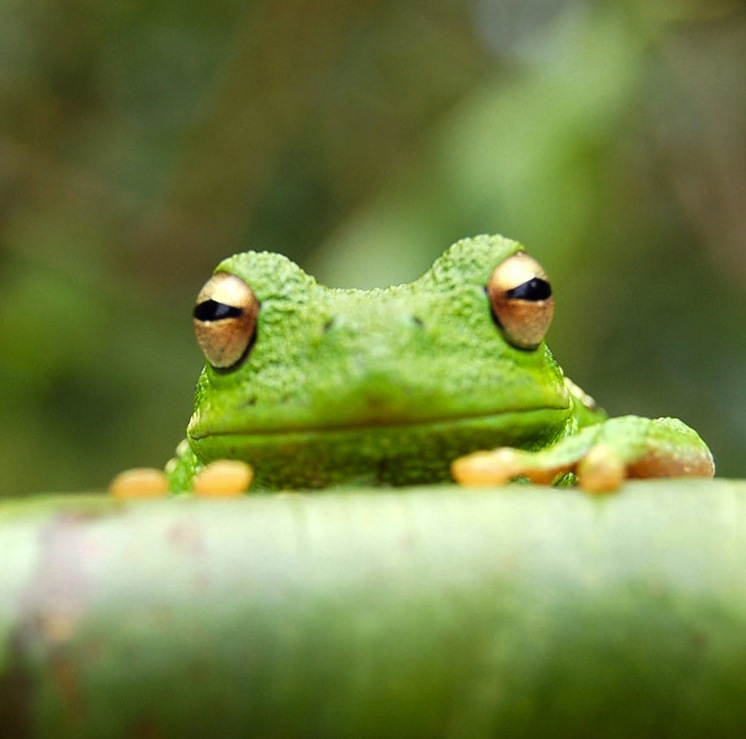
\includegraphics[width=0.3\textwidth]{frog.jpg}
%\caption{\label{fig:frog}This frog was uploaded via the project menu.}
%\end{figure}


%\begin{table}
%\centering
%\begin{tabular}{l|r}
%Item & Quantity \\\hline
%Widgets & 42 \\
%Gadgets & 13
%\end{tabular}
%\caption{\label{tab:widgets}An example table.}
%\end{table}


\bibliographystyle{abbrv}
\bibliography{thiazole}

\end{document}